\lhead[\thepage]{APÉNDICE A. SUMMARY}
\chead[]{}
\rhead[WepSIM: Simulador de un procesador elemental con unidad de control microprogramada]{\thepage}
\renewcommand{\headrulewidth}{0.5pt}

\lfoot[]{}
\cfoot[]{}
\rfoot[]{}
\renewcommand{\footrulewidth}{0pt}

\appendix
\clearpage
\addappheadtotoc
\appendixpage
\chapter{Summary}
\label{ch:apendicea}

\section*{Introduction}

Teaching the topics related to the architecture of a computer is a basic and fundamental part of the training of computer science students. In these subjects, students achieve a low-level vision and understanding of the components of a computer. In order to facilitate the correctly understanding of the theoretical foundations, it is necessary to use practical classes, where the student should interact with the architecture of a computer in a similar way to that one explained in theory and also manage to extrapolate the theoretical foundations to the actual behavior.

One of the main problems when preparing these practical classes is to emulate the necessary resources seen in the theoretical classes. Currently, there are different tools that enable the emulation of different components of a computer. However, there is a lack of tools that unify the simulation of these components, being a problem when trying to obtain a global view of the operation of a computer.

These tools can be classified into two main types: emulators and simulators. An emulator is a software that imitates the behavior of a computer, so that programs designed for a particular architecture can be executed in a different one. On the other hand, a simulator is a software that aims to reproduce the behavior of a computer, but with a lower level of realism than the emulators.

There are different simulators that can be used in order to work with the main aspects treated in the subjects of ``Computer Architecture and Computer Sctructure'' such as assembler, cache, etc. Most of these simulators are focused on a specific type of simulation, which implies that, to obtain a global vision on the architecture of the computer several simulators are needed. Therefore, it is much better to count with a tool that offers a complete simulation of the architecture and combines the maximum possible functionalities.

We identify another important problem: most of the simulators are designed for running as PC applications. One of the goals we put forward with WepSIM is that it could be used in smartphones or tablets in order to offer greater flexibility in its usage to the student.

In addition to having a portable simulator, it must also be as self-contained as possible. Therefore, it must integrate support for its use inside the tool(not as a separate document that serves as a user manual to be printed), allowing the end-user to make full use of the application without the need of getting out of it.

In conclusion, we have considered how to offer a simulator that is simple and modular, and that at the same time allows to integrate the teaching of the microprogramming language with programming in assembly. In particular, it can be used to microprogram a customized instruction set and observe the basic operation of a processor, as well as to create assembler programs based on the assembler defined by the above microcode. This is of great help, for example, for system programing, since it is possible to follow how the software interacts in assembly with the hardware in the treatment of interruptions. The idea is to offer a simulator that offers a global vision of a computer, integrating both hardware and software components and also avoiding the extra time involved in learning different tools.


\section*{Objectives}

The main objective of this project is to design and develop a simulator, which, unlike the existing ones, can fully simulate the behavior of an elementary processor allowing to check the state of the components in each clock cycle, so that it helps the students to understand and assimilate in a simple and visual way the operation of a processor. The secondary objectives, derived from the main objective, are as follow:

\begin{itemize}

\item \textbf{O1:} Simulate the execution of the set of instructions specified in a computer called WepSIM from the point of view of microprogramming and programming in assembly.

\item \textbf{O2:} Allow the specification of different and customized sets of instructions.

\item \textbf{O3:} Allow unified microprogramming in a computer and programming in assembly language.


\item \textbf{O4:} Allow the user to display in each clock cycle the status and behavior of the simulated computer.

\end{itemize}

\section*{WepSIM Elemental Processor}

WepSIM is an elementary processor with an integrated microprogrammed control unit designed by the staff of the research group ARCOS of the University Carlos III of Madrid. This processor design is used for teaching in the subject ``Computer Structure''.

In Figure \ref{fig:wepsimCPU_figure_summary}, the structure of the WepSIM Elemental Processor is shown. WepSIM consists of a memory module, a keyboard device, a display device, and a generic I/O device that can be used to work with interrupts.

\begin{figure}[htbp]
 	\centering
 	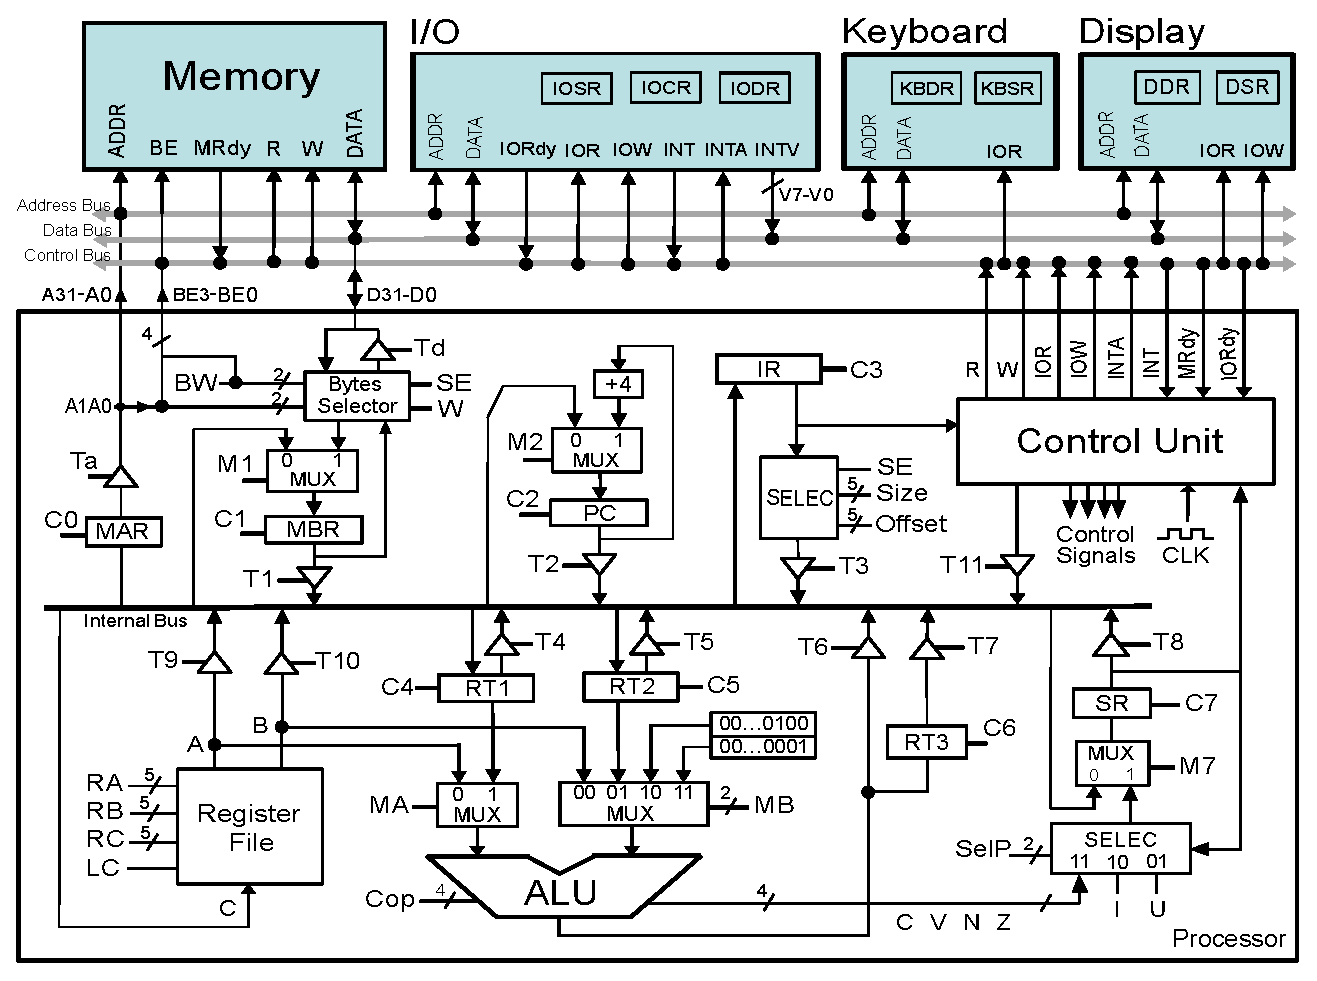
\includegraphics[width=11cm]{figures/processor6}
 	\caption{CPU Architecture WepSIM.}
	\label{fig:wepsimCPU_figure_summary}
\end{figure}

\begin{figure}[htbp]
 	\centering
 	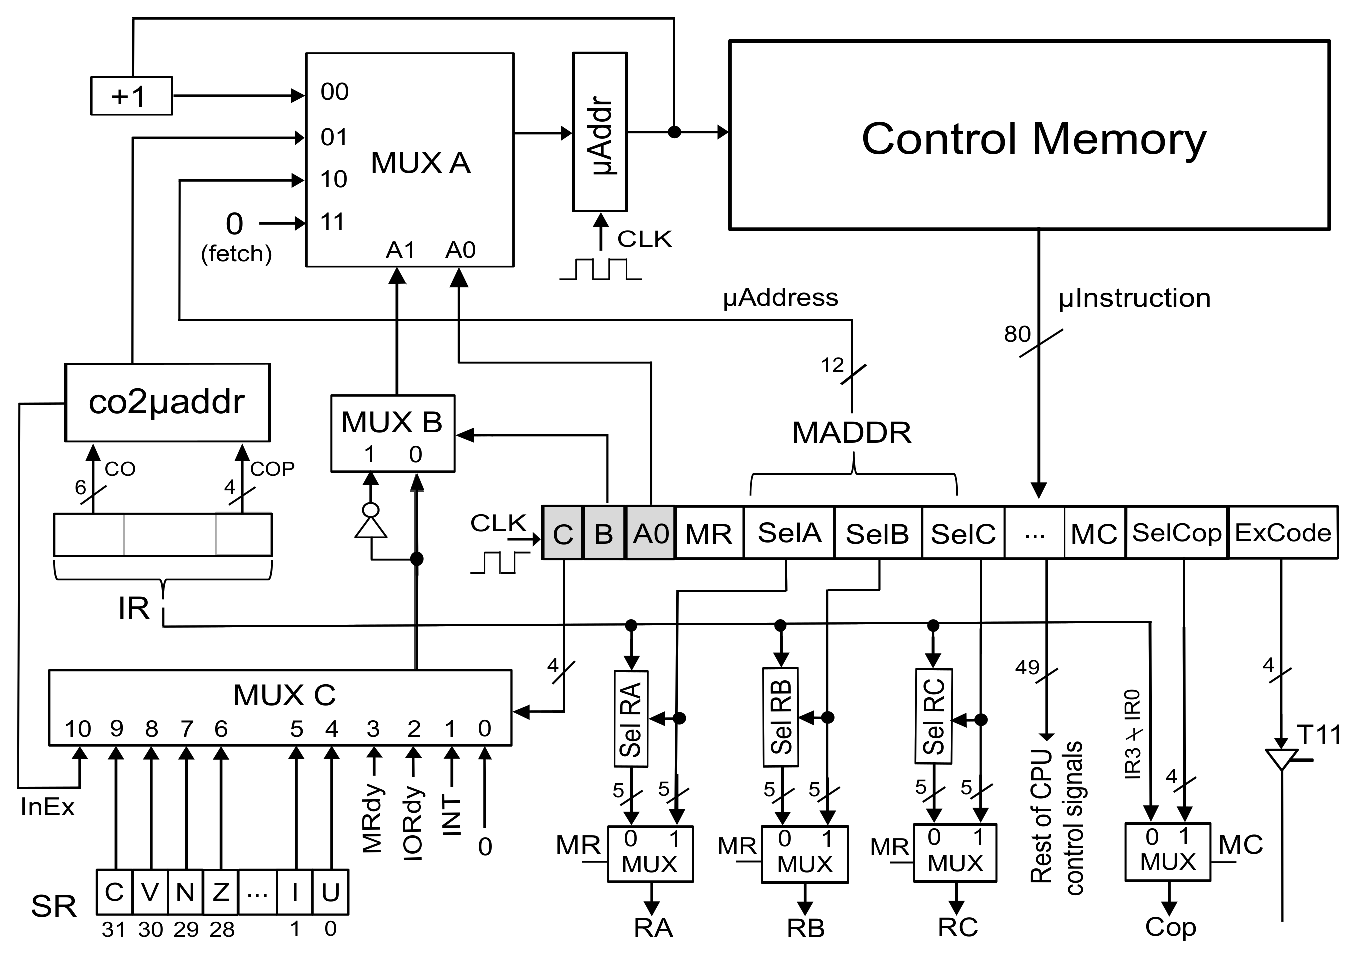
\includegraphics[width=11cm]{figures/controlunit6}
 	\caption{Control unit architecture in WepSIM.}
	\label{fig:wepsimCU_figure_summary}
\end{figure}


WepSIM incorporates a 32bit processor that includes a byte addressable memory,  a bank of 32 registers and two additional registers (\emph{RT1 and RT2}) that are not visible to the assembly programmer but allow temporary storage of data for the carrying out of intermediate operations. From the registers, it is possible to forward the values to operate in an \emph{ALU} that implements the 15 most common arithmetic-logic operations. The \emph{PC} registry has its own 4-add operator, so it is not necessary to make use of the \emph{ALU} for this operation. The result of the operations performed in the \emph{ALU} can be stored in a temporary register (\emph{RT3}) that is also invisible to the assembly programmer, or sent directly to the internal bus through the corresponding tristate.


The status register \emph{(SR)} can be updated with the resulting flags of the last operation of the \emph{ALU (O, N and Z)}. To do this, \emph{SELEC/SelP} represents a circuit block that allows indicating which part of the state register (\emph{SR}) must be updated. To the right of \emph{SELEC/SelP} the bits of the \emph{SR} status register enter (\emph{Input = ONZIU}) and \emph{SelP} allows to select which group of these bits will be updated in the status register: bits \emph{O, N and Z} with the values coming of the \emph{ALU}, the bit I with the indicated value or the bit \emph{U} with the indicated value for the same.

The instruction register (\emph{IR}) is associated with a selector module (higher level circuit than a multiplexer, etc.), which allows the selection of a segment of the binary value stored in the instruction register that will pass to \emph{T3}.

In particular, the position (offset, where 0 represents the least significant bit of the \emph{IR} register) and the number of bits (\emph{Size}) to be taken from that initial position is indicated, and wether if sign extension (\emph{SE}) is desired before passing the value to the \emph{T3} input.

The \emph{MAR} and \emph{MBR} registers are used to store the address and content associated with this address in read/write operations with memory. The memory is designed for synchronous or asynchronous operation. It currently works synchronously, but has the \emph{MRdy} signal for working asynchronously in the future. The selection circuit allows the user to indicate which portion of the memory word is the desired one (one byte, two bytes, or a complete four-byte word).

There are also three I / O devices: a keyboard, a display and a generic device that can be configured to generate various types of interrupts.

Finally, the Control Unit generates the control signals for each clock cycle. The Figure \ref{fig:wepsimCU_figure_summary} shows the Control Unit in more detail. It is a microprogrammed control unit with implicit sequencing. The control signals for the current clock cycle are stored in the micro-instruction register (the one with the fields \emph{A0, B, C, SelA}, etc.). The contents of this record come from the control memory, specifically from the content in the position to which the micro-address register points. The micro-address stored in this register can be modified using the ``MUX'' multiplexer. There are four options: the current micro-address plus one, a micro-address indicated in the micro-instruction itself (which overlaps with \emph{SelA, SelB} and partially with \emph{SelE}), the first micro-address associated with the operation code field of the instruction of the \emph{IR} register, and finally the value zero, which is the address of the control memory where the microprogram corresponding to the fetch is stored. The micro address can be selected conditionally by using the ``MUX C '' multiplexer that allows to select the status register bits (SR) or values of the I/O control signals. 

The \emph{SelRA, SelRB and SelRE} selector circuits are used to generate the values corresponding to the selector signals of the register bank \emph{RA, RB and RE}. These selectors take as input the 32 bits of the instruction register (\emph{IR}) on one side and the field \emph{SelA, SelB and SelE} on the other, so that they take \emph{SelX} as the displacement within the instruction register (from 0 to 32) from where Take the next 5 bits corresponding to the \emph{RA, RB or RE} signals. They thus allow to select 5 consecutive bits of the 32 bits of the instruction register.

The MR multiplexer is used to indicate whether the \emph{RA, RB and RE} signals are literally the values stored in \emph{SelA, SelB and SelE} (MR = 1) or if \emph{SelA, SelB and SelE} indicate the offset within the instruction where the values to be used for \emph{RA, RB and RE}. The latter allows the instruction to indicate the registers to be used as operands in the register bank, instead of indicating them from the micro-instruction.

For the \emph{Cop} signal (operation code in the \emph{ALU}), the \emph{MC} signal can be used to take the \emph{SelCop} value of the micro-instruction (\emph{MC} = 1) or the 4 least significant bits of the instruction register (MC = 0), ie \emph{IR3 -IR0}.

\section*{Simulator design}

In order for the teachers of the Computer Structure subject to use a tool that helps to explain the theoretical concepts of the subject, and that, at the same time, students can employ to understand the main concepts and to carry out the subject's practices later we propose the design and implementation of a web tool that realistically simulates an elementary processor with a microprogrammable control unit.

This simulator will be developed as a web tool due to the portability it provides, since it can be executed on a large number of different devices regardless of the operating system use, only needing a web browser for its correct operation. In this way, teachers and students will be able to use the tool without depending on their installation in the device to be used, even allowing the students to practice on mobile devices.

To achieve this portability, the simulator has been developed in HTML5 (HTML + JavaScript + CSS) making it possible to run on any platform (smartphones, tablets, PC, etc.) being compatible with Microsoft Edge, Mozilla Firefox, Google Chrome or Safari. In addition, the tool depends on the following frameworks or libraries: JQuery, JQueryUI, JQuery Mobile, Knockout, and BootStrap.

Therefore, the chosen solution is able to unify in a single tool all the features required for the teaching of Computer Structure with a high level of detail, with high availability by facilitating it as a web tool, and being portable, since it an be executed on a large number of different devices, always looking for a solution without the need for a server.

\subsection*{Simulator Architecture}

The architecture of the solution presented in this work consists of three main elements:

\begin{itemize}
\item \textbf{Hardware model:} allows the user to define the hardware to use.
\item \textbf{Software model:} allows the user to define the set of instructions to use.
\item \textbf{Simulation kernel:} simulates hardware operation by running the microcode / machine language previously defined.
\end{itemize}

The hardware model allows the user to define the typical elements of a computer (main memory, processor, etc.) in a modular way. The way in which these elements are defined balances two opposing objectives: it must be complete enough to imitate the main aspects of reality, but also minimal enough to facilitate its use. Above all, it is intended to be a didactic tool.

The software model allows defining the microcode and assembler based on this microcode as intuitively as possible. The assembly used is given by a set of instructions that can be defined by the user.These instructions try to be flexible enough to be able to define different types and sets of instructions, such as MIPS or ARM.

The third element of the proposed architecture is a kernel that takes as input the described hardware model and the working software model, and is responsible for showing the operation of the hardware with the given software.

\begin{figure}[htbp]
 	\centering
 	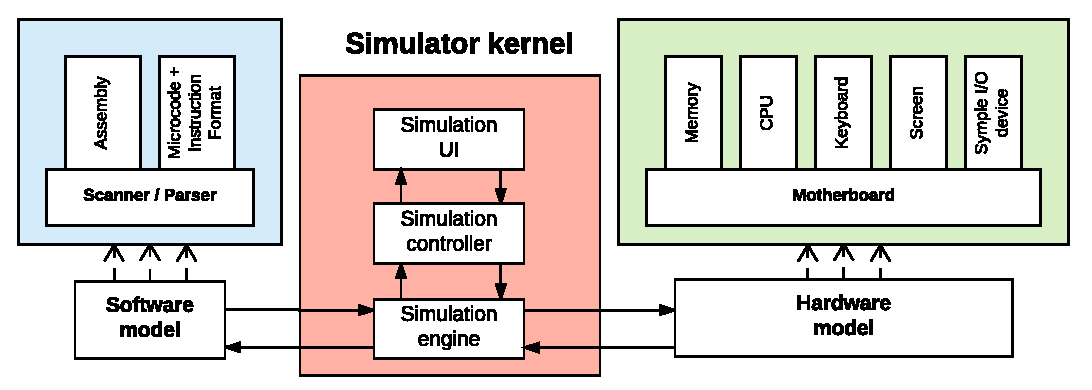
\includegraphics[width=14cm]{figures/architecture_diagram}
 	\caption{WepSIM Architecture.}
	\label{fig:architecture_diagram_summary}
\end{figure}

Figure \ref{fig:architecture_diagram_summary} summarizes the architecture of WepSIM. The starting point is the hardware model that describes the processor to be simulated. This includes the processor, memory, and some I/O devices such as keyboard, display, and a single I/O device that generates interrupts. The hardware model describes the overall state of the processor. From the processor's overall state, the simulation kernel updates the state in each clock cycle.

The simulated control unit stores the control signals of each cycle in a control memory. The control memory has all the microprograms for the instructions with which the processor works, and the fetch instruction to be able to read the instructions from the memory and to decode them.

The microcode (the contents of the control memory) together with the format of each instruction (fields of the instruction and its length) is described in a text file. The software model reads this file, translates it to binary and loads it into the processor. The definition of the assembly language to be used is described together with the microcode, and the software model allows to translate programs written in said assembler to binary.


The simulation kernel asks the subsystem of the software model for the defined microcode, the description of the instruction format and the contents of the main memory. The binaries are loaded into the elements of the hardware model, and then the simulation kernel updates the global state in each clock cycle.

WepSIM has a simulation controller that is responsible for updating the clock cycle and displaying the global status. The simulation interface subsystem updates the user interface. When the user uses the user interface to request an operation, the simulation interface subsystem moves the request to the simulation controller. In this way, a basic Model-View-Controller (MVC) design is used for the WepSIM architecture.

\section*{Conclusions and future work}

This section presents the conclusions obtained from the project, reviews the objectives set out at the beginning of this document, and includes some personal observations. In addition, we discuss the main contributions of our work, also indicating the publications resulting from this project. Finally, future work is discussed.

\section*{Conclusions}

In this work, we have described the design of WepSIM, an elementary processor simulator with a microprogrammed control unit. This work presents a new simulator that is intuitive, portable and extensible, serving as a teaching complement for teaching in Computer Structure. This simulator enables the definition of different sets of instructions and the execution and debugging of source code. It also allows to define the behavior of the processor by microprogramming instructions, also defined by the end-users.

WepSIM allows students to understand the operation of an elementary processor in a simple way, can be used from a mobile device or a computer with a modern Web browser without the need of being installed. In this way, students can interact with the simulator by learning and understanding the operation of the WepSIM elementary processor, including the mechanisms of interaction with the system software and integrating in the same tool both the microprogramming and the programming in assembler.

The main objective of this project was to develop a simulator, which, in contrast to existing ones, could completely simulate the behavior of an elementary processor, allowing to check the state of the components in each clock cycle, so that students understand and assimilate in a simple and visual way the operation of a processor. We have also met all the other objectives presented in the introduction of the document:

\begin{itemize}

\item \textbf{O1}, A tool has been designed that simulates the execution of the instruction set specified in a computer called WepSIM, from the point of view of microprogramming and assembly programming.

\item \textbf{O2}, The tool allows the specification of different instructions.

\item \textbf{O3}, The tool unifies the microprogramming of a computer and programming in assembly language.

\item \textbf{O4}, The tool allows the user to display in each clock cycle the state and behavior of the simulated computer.

\end{itemize}

On a personal level, this work has helped me to enter the world of scientific research. I have been able to apply a great deal of the knowledge acquired throughout the degree. In addition, I have learned important techniques of hardware modeling, compilation and simulation, which have a great utility and complexity and have served me to deepen even more in the knowledge acquired in the degree. For all this, it is very satisfying to see the final result obtained, since I have managed to overcome all the problems that have arisen throughout the project.

\subsection*{Contributions}

The project carried out during this Bachelor Thesis fits with many of the subjects studied in the Degree in Computer Engineering of the University Carlos III of Madrid, highlighting the following topics in particular:

\begin{itemize}

\item \textbf{Computer technology} (Compulsory subject, First course) Where the hardware components and binary logic are introduced.

\item \textbf{Computer structure} (Compulsory subject, Second course) Where the bases of the structure and operation of a computer are introduced.

\item \textbf{Formal languages and Automata theory} (Compulsory subject, Second course) Where the bases are introduced about the formal languages and grammars.

\item \textbf{Operating systems} (Compulsory subject, Second course) Where the bases of the operation of the operating system are introduced.

\item \textbf{Computer architecture} (Compulsory subject, Third course) Where the bases of the architecture of a computer are introduced.

\item \textbf{Operating systems design} (Compulsory subject, Third course) Where the bases of the design of the different modules of an operating system are introduced.

\item \textbf{Software development projects management} (Compulsory subject, Third course) Where the bases for the management and management of a software development project are introduced.

\end{itemize}

\subsection*{Publications}

This bachelor thesis has permitted to make an important contribution to the field of teaching in Structure and Computer Architecture. In addition, the following scientific articles have been published:

\begin{itemize}

\item \textbf{A. Calderón, F. García-Carballeira, and J. Prieto}, “WepSIM: Simulador modular e interactivo de un procesador elemental para facilitar una visión integrada de la microprogramación y la programación en ensamblador”, \textit{Enseñanza y aprendizaje de ingeniería de computadores}, vol. 6, 35-53,2016. \cite{mateos2016wepsim}

\item \textbf{J. Prieto, A. Calderón, F. García-Carballeira, and S. Alonso-Monsalve}, “WepSIM: simulador integrado de microprogramación y programación en ensamblador”, \textit{Jornadas sarteco 2016}. \cite{arcos2032}

\end{itemize}

In addition, at the time of delivery of this document, there is also another item sent waiting for its acceptance.

\clearpage

\section*{Future works}

Currently, there are many lines of future work in which we are working on:

\begin{itemize}

\item Regarding improvements in the hardware model:

\begin{itemize}

\item[1.] Introduce more hardware elements, such as a cache, in order to expand the contents of the subject included in the tool.

\item[2.] Introduce a hardware model based on a pipeline, allowing the use of the tool in those subjects that employ this architecture model.

\end{itemize}

\item Regarding improvements in the software model:

\begin{itemize}

\item[3.] Add semantic revision of the code, allowing to identify and notify the programming errors to the user.

\item[4.] Add new sets of instructions to the tool such as the ARM assembler, allowing the use of different languages in the tool.

\item[5.] Study the MIPS / ARM assembler generated with GCC/Clang so that it can be used directly in WepSIM.

\end{itemize}

\item Regarding improvements in the tool:

\begin{itemize}

\item[6.] Add an automatic correction module for practices to the tool, so that students can practice with it and check the validity of their exercises.

\item[7.] Migrate the tool to a mobile application using the Apache Cordova plugin, so that the tool is not limited to its usage in a web browser.

\end{itemize}

\end{itemize}

